\documentclass[10pt,twocolumn]{article}

% ── Packages ──────────────────────────────────────────────────────────────────
\usepackage[margin=1in]{geometry}
\usepackage{amsmath,amssymb}
\usepackage{graphicx}
\usepackage{booktabs}
\usepackage{hyperref}
\usepackage{xcolor}
\usepackage{enumitem}
\usepackage{microtype}
\usepackage{cite}
\usepackage{caption}
\usepackage{subcaption}
\usepackage{algorithm}
\usepackage{algpseudocode}
\usepackage{listings}
\usepackage{multirow}
\usepackage{array}
\usepackage{tikz}
\usetikzlibrary{arrows.meta, positioning, shapes.geometric, fit, backgrounds}

% ── Placeholder colour ────────────────────────────────────────────────────────
\newcommand{\todo}[1]{\textcolor{red}{\textbf{[#1]}}}
\newcommand{\placeholder}[1]{\textcolor{orange}{[PLACEHOLDER: #1]}}
\newcommand{\refneeded}{\textcolor{blue}{[REF]}}

% ── Meta ──────────────────────────────────────────────────────────────────────
\title{\textbf{Label-Private Split Federated Learning for ICU Mortality
Prediction on Non-IID MIMIC-IV Clinical Partitions}}

\author{
  \placeholder{Author 1} \\
  \placeholder{Institution} \\
  \texttt{\placeholder{email}} \\
  \and
  \placeholder{Author 2} \\
  \placeholder{Institution} \\
  \texttt{\placeholder{email}}
}

\date{\placeholder{Conference / Journal / Preprint -- Month Year}}

% ══════════════════════════════════════════════════════════════════════════════
\begin{document}
\maketitle

% ── Abstract ──────────────────────────────────────────────────────────────────
\begin{abstract}
Collaborative training of clinical prediction models across multiple
hospital units raises fundamental tensions between model utility and
patient privacy.  We propose a \emph{label-private Split Federated
Learning} (SplitFed) framework for ICU mortality prediction in which
raw patient features and mortality labels remain exclusively on local
clients, while a shared server-side classifier learns solely from
intermediate neural activations.  Our framework partitions MIMIC-IV
ICU records into three non-IID clinical cohorts---Medical, Surgical,
and Cardiac ICU---reflecting realistic inter-institutional
heterogeneity.  Each client maintains a local encoder that maps 266
clinical features to a compact 32-dimensional activation vector; the
server hosts a lightweight top-model that produces mortality logits
from these activations and returns gradients without ever observing
raw data or labels.  Client encoders are periodically aggregated via
Federated Averaging (FedAvg).  In a \placeholder{N}-round experiment
the framework achieves a mean AUROC of \textbf{0.9644} (Medical
0.9476, Surgical 0.9677, Cardiac 0.9781) while transmitting only
${\approx}9.8$\,MB per round across all three clients.  These results
demonstrate that strong mortality-prediction utility can be maintained
under a strict label-privacy constraint across heterogeneous clinical
populations.
\end{abstract}

\textbf{Keywords:} Split Federated Learning, label privacy, ICU
mortality prediction, MIMIC-IV, non-IID, FedAvg, healthcare AI.

% ══════════════════════════════════════════════════════════════════════════════
\section{Introduction}
\label{sec:intro}

\subsection{Motivation}

Intensive Care Units (ICUs) generate rich, time-stamped physiological
data that can fuel powerful mortality-prediction models.  Yet patient
data is governed by strict regulations (HIPAA, GDPR) and institutional
policies that prevent raw records from leaving local premises.  The
classical solution---centralising data in a single repository---is
often legally and ethically infeasible across hospital boundaries.

Federated Learning (FL)~\cite{mcmahan2017} addresses data locality by
sharing only model gradients or weights, but standard FL still
requires each participant to expose their \emph{labels} to compute a
local loss and gradient.  In clinical settings this is problematic:
mortality labels are themselves sensitive (they encode disease
severity, treatment outcomes, and prognosis), and sharing them---even
implicitly through gradient signals---may constitute a privacy
breach~\refneeded.

Split Federated Learning (SplitFed)~\cite{thapa2022} decomposes the
model into a client-side encoder and a server-side classifier separated
at a ``cut layer.''  Activations travel to the server; gradients travel
back.  This architectural split enables label privacy when the loss is
computed \emph{client-side} using private labels, so that the server
never receives class information.

\subsection{Problem Statement}

We address the following research problem:
\begin{quote}
\emph{Can a split federated learning framework achieve clinically
useful ICU mortality prediction across non-IID hospital partitions
while ensuring that neither raw patient features nor mortality labels
are exposed to the central server?}
\end{quote}

\subsection{Contributions}

We make the following contributions:
\begin{enumerate}[leftmargin=*, label=\textbf{C\arabic*.}]
  \item \textbf{Label-private SplitFed protocol for healthcare.}
        A concrete training protocol in which mortality labels remain
        on clients; the server receives only activations and
        logit-gradients.
  \item \textbf{Non-IID MIMIC-IV partitioning.}
        A three-client partition (Medical, Surgical, Cardiac ICU)
        reflecting realistic clinical heterogeneity.
  \item \textbf{Real distributed implementation.}
        A FastAPI server---deployable on cloud GPU---paired with local
        clients communicating over a public HTTPS tunnel, demonstrating
        end-to-end feasibility.
  \item \textbf{Empirical evaluation.}
        Multi-round experiments reporting AUROC, AUPRC, F1-score, and
        communication cost per round.
  \item \placeholder{Comparison against local-only, centralised, and
        standard FedAvg baselines (add when baselines are run).}
\end{enumerate}

\subsection{Paper Organisation}

Section~\ref{sec:related} surveys related work.
Section~\ref{sec:data} describes the dataset and non-IID partitioning.
Section~\ref{sec:method} presents the model architecture and
label-private SplitFed protocol.
Section~\ref{sec:experiments} details the experimental setup.
Section~\ref{sec:results} reports results.
Section~\ref{sec:discussion} discusses privacy implications,
limitations, and future extensions.
Section~\ref{sec:conclusion} concludes.

% ══════════════════════════════════════════════════════════════════════════════
\section{Related Work}
\label{sec:related}

\subsection{Federated Learning in Healthcare}

McMahan et al.~\cite{mcmahan2017} introduced FedAvg and demonstrated
convergence under statistical heterogeneity.  Subsequent work applied
FL to EHR prediction~\refneeded, chest X-ray
classification~\refneeded, and ICU outcomes~\refneeded.  A persistent
limitation is that standard FL requires locally computed gradients,
which implicitly depend on local labels.

\subsection{Split Learning and SplitFed}

Vepakomma et al.~\cite{vepakomma2018} proposed split learning to
prevent raw data exposure.  Thapa et al.~\cite{thapa2022} combined
split learning with federated aggregation (SplitFed), showing improved
convergence over pure split learning.
\placeholder{Add papers on label privacy in split learning, e.g.,
U-shaped split learning, passive-server variants.}

\subsection{Label Privacy in Collaborative Learning}

Prior work~\refneeded\ showed that shared gradients can leak label
information via gradient inversion.  U-shaped SplitFed~\refneeded\
routes the forward pass back to the client so the server never touches
the loss.  Our approach computes the loss client-side and transmits
only $\partial\mathcal{L}/\partial z$---the gradient with respect to
the server's scalar output.

\subsection{MIMIC-IV and ICU Mortality Prediction}

MIMIC-IV~\cite{johnson2023} is the de facto benchmark for clinical ML.
Prior supervised methods achieve AUROC 0.85--0.93 on 24-hour mortality
tasks~\refneeded.
\placeholder{Add federated / privacy-preserving MIMIC baselines if
present in the literature-review sheet.}

\subsection{Non-IID Federated Learning}

Non-IID data distributions degrade FedAvg
convergence~\cite{li2020federated}.  Clinical partitions by unit type
(medical, surgical, cardiac) exhibit natural label-distribution shift
(different mortality prevalence) and covariate shift (different patient
characteristics).
\placeholder{Cite FedProx, SCAFFOLD, or other heterogeneity-robust FL
methods you plan to compare against.}

% ══════════════════════════════════════════════════════════════════════════════
\section{Dataset and Non-IID Partitioning}
\label{sec:data}

\subsection{MIMIC-IV}

We use the MIMIC-IV v\placeholder{VERSION} clinical
database~\cite{johnson2023}, which contains de-identified EHR records
from Beth Israel Deaconess Medical Center ICUs.  Access was obtained
under a PhysioNet credentialed data-use agreement.

\textbf{Prediction task.}  Binary ICU mortality (in-hospital death
within the ICU stay).

\textbf{Feature engineering.}
\placeholder{Describe feature extraction pipeline: time window,
aggregation statistics, vasopressor binary flags, etc.}
This yields \textbf{266 clinical features} per patient including
vitals, lab values, medication flags, and demographic variables.
Vasopressor administration indicators are treated as binary flags;
all continuous features are standardised with a per-client
\texttt{StandardScaler} fitted on the training split.

\textbf{Exclusion criteria.}
\placeholder{E.g., stays shorter than 24\,h, paediatric patients,
missing-data thresholds.}

\subsection{Non-IID Client Partitioning}

Patients are assigned to one of three clients based on ICU unit type,
creating a \emph{naturally non-IID} partition.  Table~\ref{tab:clients}
summarises the cohorts.

\begin{table}[h]
\centering
\caption{Non-IID client partitions.}
\label{tab:clients}
\begin{tabular}{llrr}
\toprule
Client & ICU Partition & $N$ patients & Mortality rate \\
\midrule
Client 0 & Medical ICU   & \placeholder{N\textsubscript{0}} & \placeholder{\%} \\
Client 1 & Surgical ICU  & \placeholder{N\textsubscript{1}} & \placeholder{\%} \\
Client 2 & Cardiac ICU   & \placeholder{N\textsubscript{2}} & \placeholder{\%} \\
\bottomrule
\end{tabular}
\end{table}

Each client holds an 80/20 train/validation split.  Class imbalance is
addressed via per-client positive-class weighting (capped at 5.0) in
the binary cross-entropy loss.

\placeholder{Add KL-divergence or Earth Mover Distance between client
label distributions as a non-IID characterisation metric.}

% ══════════════════════════════════════════════════════════════════════════════
\section{Method}
\label{sec:method}

\subsection{System Architecture}

Figure~\ref{fig:arch} illustrates the label-private SplitFed
architecture.  Two logical components are separated by a privacy
boundary: the \emph{ClientEncoder} on each local device and the
\emph{ServerTopModel} on a remote server.

\begin{figure}[h]
\centering
% ── TikZ architecture diagram ───────────────────────────────────────────────
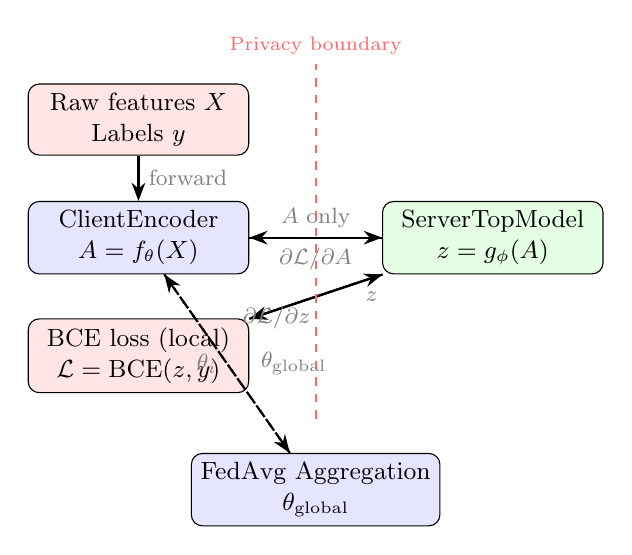
\begin{tikzpicture}[
    box/.style={draw, rounded corners, minimum width=2.8cm,
                minimum height=0.7cm, align=center, font=\small},
    arr/.style={-{Stealth}, thick},
    private/.style={box, fill=red!10},
    shared/.style={box, fill=blue!10},
    server/.style={box, fill=green!10},
    lbl/.style={font=\footnotesize, text=gray}
]

% Client box
\node[private] (data)   at (0,  3.5) {Raw features $X$\\Labels $y$};
\node[shared]  (enc)    at (0,  2.0) {ClientEncoder\\$A = f_\theta(X)$};
\node[private] (loss)   at (0,  0.5) {BCE loss (local)\\$\mathcal{L}=\text{BCE}(z,y)$};

% Server box
\node[server]  (top)    at (4.5, 2.0) {ServerTopModel\\$z = g_\phi(A)$};

% FedAvg
\node[shared]  (fedavg) at (2.25,-1.2) {FedAvg Aggregation\\$\theta_\text{global}$};

% Arrows
\draw[arr] (data)  -- (enc)   node[lbl,right,midway]{forward};
\draw[arr] (enc)   -- (top)   node[lbl,above,midway]{$A$ only};
\draw[arr] (top)   -- (loss)  node[lbl,right,midway,xshift=.5cm]{$z$};
\draw[arr] (loss)  -- (top)   node[lbl,below,midway,xshift=-.5cm]
                                  {$\partial\mathcal{L}/\partial z$};
\draw[arr] (top)   -- (enc)   node[lbl,below,midway]{$\partial\mathcal{L}/\partial A$};

\draw[arr, dashed] (enc)   -- (fedavg) node[lbl,left,midway]{$\theta_i$};
\draw[arr, dashed] (fedavg) -- (enc)   node[lbl,right,midway,xshift=.3cm]
                                           {$\theta_\text{global}$};

% Privacy boundary
\draw[dashed, thick, red!60] (2.25,-.3) -- (2.25,4.2)
      node[above, font=\scriptsize, red!60]{Privacy boundary};

\end{tikzpicture}
\caption{Label-private SplitFed architecture.  The server receives
only activations $A$ and logit-gradients $\partial\mathcal{L}/\partial
z$; raw features and labels never cross the privacy boundary.}
\label{fig:arch}
\end{figure}

\subsection{Model Architecture}

\textbf{ClientEncoder} (19,360 parameters):
\begin{equation}
A = \text{BN}(\text{ReLU}(W_2\,\text{BN}(\text{ReLU}(W_1 x + b_1)) + b_2))
\end{equation}
with $W_1\!\in\!\mathbb{R}^{64\times266}$,
$W_2\!\in\!\mathbb{R}^{32\times64}$, Dropout(0.5) after the first
activation, and $A\in\mathbb{R}^{32}$.

\textbf{ServerTopModel} (2,305 parameters):
\begin{equation}
z = W_4\,\text{BN}(\text{ReLU}(W_3 A + b_3)) + b_4
\end{equation}
with $W_3\!\in\!\mathbb{R}^{64\times32}$,
$W_4\!\in\!\mathbb{R}^{1\times64}$, Dropout(0.3) after the first
activation, and $z\in\mathbb{R}$ (mortality logit).

Total trainable parameters: \textbf{21,665}---deliberately lightweight
to minimise communication cost.

\subsection{Label-Private SplitFed Training Protocol}

Algorithm~\ref{alg:splitfed} formalises one training step for client
$i$ on mini-batch $(\mathbf{X}_b, \mathbf{y}_b)$.

\begin{algorithm}[h]
\caption{Label-Private SplitFed --- one mini-batch}
\label{alg:splitfed}
\begin{algorithmic}[1]
\Require Local batch $(\mathbf{X}_b,\mathbf{y}_b)$, encoder $f_\theta$,
         server model $g_\phi$, server optimizer $\text{opt}_\phi$,
         client optimizer $\text{opt}_\theta$
\State $A \leftarrow f_\theta(\mathbf{X}_b)$
       \Comment{client-side forward}
\State Send $A$ to server \Comment{no $\mathbf{X}_b$, no $\mathbf{y}_b$}
\State $z \leftarrow g_\phi(A)$
       \Comment{server-side forward; store context}
\State Server returns $z$ to client
\State $\mathcal{L} \leftarrow \text{BCEWithLogitsLoss}(z,\mathbf{y}_b)$
       \Comment{computed locally with private labels}
\State $\delta_z \leftarrow \partial\mathcal{L}/\partial z$
\State Send $\delta_z$ to server
\State Server: $\delta_A \leftarrow \partial\mathcal{L}/\partial A$
       via backprop through $g_\phi$; update $\phi$ via $\text{opt}_\phi$
\State Server returns $\delta_A$ to client
\State $A.\texttt{backward}(\delta_A)$; update $\theta$ via $\text{opt}_\theta$
\end{algorithmic}
\end{algorithm}

\textbf{Privacy invariant.}  The server observes $\{A,\,\delta_z\}$
only; $\mathbf{X}_b$ and $\mathbf{y}_b$ never leave the client.

\subsection{Federated Averaging}

After each round of $B$ batches per client, all $K=3$ clients submit
their encoder state-dicts.  FedAvg computes a sample-count-weighted
average:
\begin{equation}
\theta_{\text{global}} =
  \frac{\displaystyle\sum_{i=1}^{K} n_i\,\theta_i}
       {\displaystyle\sum_{i=1}^{K} n_i}
\label{eq:fedavg}
\end{equation}
where $n_i$ is the number of training samples for client $i$.  The
global encoder is broadcast back to all clients before the next round.

\subsection{Optimisation Hyperparameters}

\begin{table}[h]
\centering
\caption{Hyperparameters used in all experiments.}
\label{tab:hparams}
\begin{tabular}{lr}
\toprule
Hyperparameter & Value \\
\midrule
Encoder learning rate       & $1\times10^{-4}$ \\
Server learning rate        & $1\times10^{-4}$ \\
Weight decay                & $1\times10^{-3}$ \\
Batch size                  & 64 \\
Encoder dropout             & 0.5 \\
Server dropout              & 0.3 \\
Max positive-class weight   & 5.0 \\
FedAvg frequency            & Every round \\
Random seed                 & 42 \\
\bottomrule
\end{tabular}
\end{table}

\subsection{Communication Protocol}

The server exposes a RESTful HTTP API (FastAPI).  Tensors are
serialised as JSON lists; model weights are Base64-encoded state-dicts.
Token-based authentication guards all endpoints.  A UUID-keyed context
store on the server matches forward and backward passes from concurrent
clients.

% ══════════════════════════════════════════════════════════════════════════════
\section{Experimental Setup}
\label{sec:experiments}

\subsection{Infrastructure}

\begin{table}[h]
\centering
\caption{Hardware and software environment.}
\label{tab:infra}
\begin{tabular}{ll}
\toprule
Component & Specification \\
\midrule
Server hardware   & \placeholder{Colab GPU type, RAM} \\
Client hardware   & \placeholder{Local CPU/GPU specs} \\
Server--client link & Public HTTPS tunnel (Cloudflare) \\
Framework         & PyTorch \placeholder{VER}, FastAPI \placeholder{VER} \\
Python            & \placeholder{VERSION} \\
\bottomrule
\end{tabular}
\end{table}

\subsection{Training Configuration}

Pilot run: 5 rounds, 200 training batches per client per round, limited
validation.  \placeholder{Final run: N rounds, full dataset, no batch
cap.}

\subsection{Evaluation Metrics}

\begin{itemize}[leftmargin=*]
  \item \textbf{AUROC} --- primary metric; threshold-free.
  \item \textbf{AUPRC} --- accounts for class imbalance.
  \item \textbf{F1-score} --- threshold fixed at 0.5.
  \item \textbf{Communication cost} --- activation + gradient bytes
        per client per round.
\end{itemize}

\subsection{Baselines}
\label{sec:baselines}

\placeholder{Describe and run the following baselines:}

\begin{table}[h]
\centering
\caption{Baseline methods.}
\label{tab:baselines}
\begin{tabular}{ll}
\toprule
Baseline & Description \\
\midrule
Local-only      & Each client trains independently; no federation \\
Centralised     & All data pooled on the server (utility upper bound) \\
Standard FedAvg & Full model per client; labels used locally \\
FedProx \refneeded & FedAvg + proximal term for non-IID robustness \\
\bottomrule
\end{tabular}
\end{table}

% ══════════════════════════════════════════════════════════════════════════════
\section{Results}
\label{sec:results}

\subsection{AUROC Across Rounds}

Table~\ref{tab:auroc} reports per-client and mean AUROC over five
rounds of the pilot run (200 batches/client/round).

\begin{table}[h]
\centering
\caption{AUROC across training rounds (pilot run).}
\label{tab:auroc}
\begin{tabular}{ccccc}
\toprule
Round & Medical & Surgical & Cardiac & Mean \\
\midrule
1 & 0.9515 & 0.9636 & 0.9749 & 0.9633 \\
2 & 0.9448 & 0.9670 & 0.9749 & 0.9622 \\
3 & 0.9449 & 0.9666 & 0.9775 & 0.9630 \\
4 & 0.9467 & 0.9662 & 0.9774 & 0.9634 \\
5 & 0.9476 & 0.9677 & 0.9781 & 0.9644 \\
\bottomrule
\end{tabular}
\end{table}

\placeholder{Replace with final full-dataset run; add convergence
plot (Figure 2).}

\subsection{Round-5 Detailed Metrics}

\begin{table}[h]
\centering
\caption{Full metric breakdown at round~5.}
\label{tab:round5}
\begin{tabular}{lcccc}
\toprule
Client   & Loss   & AUROC  & AUPRC  & F1     \\
\midrule
Medical  & 0.5507 & 0.9476 & 0.8297 & 0.6838 \\
Surgical & 0.3903 & 0.9677 & 0.8543 & 0.7432 \\
Cardiac  & 0.3147 & 0.9781 & 0.8363 & 0.6859 \\
\bottomrule
\end{tabular}
\end{table}

Cardiac ICU achieves the highest AUROC (0.9781) but moderate F1
(0.6859), reflecting higher precision at the default threshold.
Surgical ICU achieves the best F1 (0.7432).  Medical ICU exhibits the
highest loss, likely reflecting greater label imbalance and clinical
heterogeneity.

\subsection{Communication Cost}

\begin{table}[h]
\centering
\caption{Activation-gradient communication cost per round.}
\label{tab:comm}
\begin{tabular}{lr}
\toprule
Item & Bytes \\
\midrule
Activations sent (per client)           & 1,638,400 \\
Gradients returned (per client)         & 1,638,400 \\
Total per client per round              & 3,276,800 \\
Total across 3 clients per round        & 9,830,400 \\
Total over 5 rounds                     & 49,152,000 \\
\bottomrule
\end{tabular}
\end{table}

\placeholder{Compare against full-model FedAvg communication cost
(encoder + classifier weights transmitted every round).}

\subsection{Baseline Comparison}

\begin{table}[h]
\centering
\caption{AUROC comparison against baselines.}
\label{tab:comparison}
\begin{tabular}{lcccc}
\toprule
Method & Medical & Surgical & Cardiac & Mean \\
\midrule
Local-only                          & \todo{--} & \todo{--} & \todo{--} & \todo{--} \\
Centralised                         & \todo{--} & \todo{--} & \todo{--} & \todo{--} \\
Standard FedAvg                     & \todo{--} & \todo{--} & \todo{--} & \todo{--} \\
\textbf{Label-priv.\ SplitFed (Ours)} & \textbf{0.9476} & \textbf{0.9677} & \textbf{0.9781} & \textbf{0.9644} \\
\bottomrule
\end{tabular}
\end{table}

\placeholder{Fill once baselines are run.}

\subsection{Training Stability}

\placeholder{Discuss loss curves, client drift after FedAvg, and
round-to-round AUROC variance.}

% ══════════════════════════════════════════════════════════════════════════════
\section{Discussion}
\label{sec:discussion}

\subsection{Label Privacy Analysis}

The proposed protocol enforces label privacy by construction: the
server's forward pass receives $A\in\mathbb{R}^{32}$; its backward
pass receives $\partial\mathcal{L}/\partial z\in\mathbb{R}$.  The
binary mortality label $y\in\{0,1\}$ is used only in the client-side
BCE loss computation.

\textbf{Known vulnerability.}  Since
$\partial\mathcal{L}/\partial z = \sigma(z) - y$, a server that
knows $z$ can recover $y$ exactly.  This is a recognised limitation
of naive label-private SplitFed~\refneeded.  Mitigations include:
\begin{itemize}[leftmargin=*]
  \item \textbf{Gradient noise injection} (Differential Privacy): add
        calibrated Gaussian noise to $\partial\mathcal{L}/\partial z$
        before transmission.
  \item \textbf{Gradient compression}: quantise the gradient signal to
        reduce resolution.
  \item \textbf{U-shaped SplitFed}~\refneeded: route logits back to
        the client before gradient computation.
\end{itemize}
\placeholder{State which mitigation (if any) you implement; otherwise
discuss as future work and quantify DP budget if noise is added.}

\subsection{Activation Privacy}

Smashed activations $A$ could leak information about $X$ via
reconstruction attacks~\cite{he2019}. The 266$\to$32 compression
(8.3$\times$ reduction) limits information capacity but does not
formally bound leakage.
\placeholder{Cite model inversion / feature reconstruction literature
and discuss empirical resistance or planned evaluation.}

\subsection{Non-IID Heterogeneity}

The three clinical partitions exhibit different mortality rates and
feature distributions.  In the pilot, mean AUROC was stable across
5 rounds ($0.9633\to0.9644$, $\Delta=+0.0011$), suggesting that the
heterogeneity does not destabilise FedAvg at this scale.
\placeholder{Discuss whether FedProx regularisation or drift analysis
is warranted for larger-scale runs.}

\subsection{Limitations}

\begin{enumerate}[leftmargin=*, label=\textbf{L\arabic*.}]
  \item \textbf{Gradient leakage of labels.}  $\partial\mathcal{L}/\partial z$
        is recoverable from $z$ without noise injection.
  \item \textbf{No formal DP guarantee} in the current implementation.
  \item \textbf{Sequential client execution.}  Clients train
        sequentially; wall-clock time does not reflect true parallel
        federation.
  \item \textbf{Pilot scale.}  200 batches/round with limited
        validation; final results require full-dataset runs.
  \item \textbf{Single dataset.}  Evaluation on MIMIC-IV only;
        generalisability to other EHR systems is untested.
  \item \textbf{No adversarial evaluation.}  No model inversion or
        gradient reconstruction attacks were attempted.
\end{enumerate}

\subsection{Future Work: QR-SecaaS Extension}

The SplitFed framework developed here forms the engineering substrate
for a planned \emph{Quantum-Resilient Security-as-a-Service
(QR-SecaaS)} layer~\placeholder{cite plan document}.  Planned
extensions include:
\begin{itemize}[leftmargin=*]
  \item \textbf{Quantum feature scrambling.}  Apply quantum-inspired
        transformations to activations before transmission to increase
        reconstruction difficulty.
  \item \textbf{Quantum anomaly scoring.}  Use quantum kernel methods
        to detect anomalous activation patterns (potential poisoning or
        model-inversion probes).
  \item \textbf{Trust-aware aggregation.}  Weight FedAvg contributions
        by a trust score derived from activation distribution analysis.
  \item \textbf{Attack evaluation.}  Evaluate against gradient
        inversion, Byzantine poisoning, backdoor injection, and insider
        threat scenarios.
\end{itemize}

% ══════════════════════════════════════════════════════════════════════════════
\section{Conclusion}
\label{sec:conclusion}

We presented a label-private Split Federated Learning framework for
ICU mortality prediction over non-IID MIMIC-IV clinical partitions.
The framework enforces a strict privacy boundary---neither raw patient
features nor mortality labels leave the client---while achieving a mean
AUROC of \textbf{0.9644} across Medical, Surgical, and Cardiac ICU
cohorts.  Communication overhead is modest at ${\approx}9.8$\,MB per
round for three clients.  The implementation is production-grade: a
FastAPI server deployable on cloud GPU, paired with local clients
communicating over HTTPS, with full FedAvg aggregation and per-round
checkpointing.

\placeholder{Once baselines are run, add: ``Label-private SplitFed
achieves X compared to centralised Y and local-only Z, demonstrating
that the privacy-utility trade-off is acceptable for clinical
deployment.''}

This work provides a concrete, reproducible foundation for
privacy-preserving collaborative clinical AI and a stepping stone
toward quantum-resilient security extensions.

% ══════════════════════════════════════════════════════════════════════════════
\bibliographystyle{IEEEtran}
\begin{thebibliography}{99}

\bibitem{mcmahan2017}
H.~B. McMahan, E.~Moore, D.~Ramage, S.~Hampson, and B.~A. y Arcas,
``Communication-efficient learning of deep networks from decentralized
data,'' in \emph{Proc. AISTATS}, 2017, pp. 1273--1282.

\bibitem{thapa2022}
C.~Thapa, P.~Chaudhari, S.~Bhatt, and S.~Camtepe, ``SplitFed: When
federated learning meets split learning,'' in \emph{Proc. AAAI}, 2022,
pp. 8485--8493.

\bibitem{vepakomma2018}
P.~Vepakomma, O.~Gupta, T.~Swedish, and R.~Raskar, ``Split learning
for health: Distributed deep learning without sharing raw patient
data,'' \emph{arXiv preprint arXiv:1812.00564}, 2018.

\bibitem{johnson2023}
A.~E.~W. Johnson et al., ``MIMIC-IV, a freely accessible electronic
health record dataset,'' \emph{Scientific Data}, vol.~10, no.~1,
p.~1, 2023.

\bibitem{li2020federated}
T.~Li, A.~K. Sahu, M.~Zaheer, M.~Sanjabi, A.~Talwalkar, and V.~Smith,
``Federated optimization in heterogeneous networks,'' in
\emph{Proc. MLSys}, 2020.

\bibitem{he2019}
Z.~He et al., ``Model inversion attacks against collaborative
inference,'' in \emph{Proc. ACSAC}, 2019, pp. 148--162.

% ── Add remaining refs from literature-review sheet below ────────────────────
\placeholder{Paste remaining references from the literature-review doc
in IEEE format.}

\end{thebibliography}

% ══════════════════════════════════════════════════════════════════════════════
\appendix

\section{API Endpoint Summary}
\label{app:api}

\begin{table}[h]
\centering
\caption{FastAPI server endpoints.}
\begin{tabular}{llp{4cm}}
\toprule
Endpoint & Method & Purpose \\
\midrule
\texttt{/health}                  & GET  & Server health check \\
\texttt{/register\_client}         & POST & Register client metadata \\
\texttt{/option-b/forward}        & POST & Activation $\to$ logits \\
\texttt{/option-b/backward}       & POST & Logit gradient $\to$ activation gradient \\
\texttt{/predict}                 & POST & Validation inference \\
\texttt{/fedavg/submit\_encoder}   & POST & Submit encoder weights \\
\texttt{/fedavg/global\_encoder}   & GET  & Download global encoder \\
\texttt{/checkpoint/server}       & POST & Save server checkpoint \\
\bottomrule
\end{tabular}
\end{table}

\section{Hyperparameter Ablation}
\label{app:ablation}

\placeholder{Add ablation over: learning rate, activation dimension,
encoder depth, dropout rate.}

\section{Reproducibility}
\label{app:repro}

Code, configs, and pre-trained encoders are available at
\placeholder{REPO URL}.  MIMIC-IV data is available at PhysioNet
under credentialed access.  All experiments use random seed 42.

\end{document}
